\appendix

\section{\rep{} details}\label{app:rep}

\begin{table}[t]
\centering\small
\caption{\rep{} channel layout per joint and frame. Channels 13--16 exist on the root row only; every
(rig, joint, channel) cell is normalised with its own statistics and exactly-constant cells are
excluded from supervision.}
\label{tab:channels}
\begin{tabular}{@{}llll@{}}
\toprule
slice & content & frame & supervised on \\
\midrule
0:3   & position (XZ relative to the smoothed root, Y absolute) & world & all joints \\
3:9   & rotation, continuous 6D delta from the rest orientation & global & free-DOF joints \\
9:12  & world velocity (supervision only, never integrated) & world & all joints \\
12    & contact flag & --- & joints with contact \\
13:15 & smoothed root trajectory XZ & world & root only \\
15:17 & heading $(\cos\phi,\sin\phi)$ & world & root only, valid frames \\
\bottomrule
\end{tabular}
\end{table}


\paragraph{Validity.} Not every cell exists on every rig or frame. Frame and joint masks handle
padding; rotation is supervised only on joints with free degrees of freedom, contact only on joints
that can touch the ground, heading only on frames where it is defined. The same effective-validity
mask multiplies the interpolant, the loss and the per-step projection at sampling time, so an
invalid cell is exactly zero everywhere rather than ``small''.


\paragraph{Why standardise rather than scale.} We found this to be decisive: with the
scale-only normalisation of the source protocol the network settled on a frozen pose while the root
travelled, because a constant pose already captured most of the objective: predicting the per-cell mean
alone recovers $75\%$ of the scale-only objective on this corpus, against $36.5\%$ once every cell
is standardised, so standardisation is what leaves the network something to learn. 

\paragraph{Conversion.} A clip enters as a kinematic tree, a rest pose and per-frame local
rotations and root translation. It is first resampled to 30\,fps (linear interpolation of the root
translation, spherical interpolation of the local rotations, then forward kinematics) and expressed
in a right-handed canonical basis. Global joint rotations follow from forward kinematics; the
\emph{heading} is the ground-plane direction of the rig's forward axis carried by a designated joint,
$(\cos\phi,\sin\phi)$ with $\phi$ measured from $+Z$, and is marked invalid (channels set to zero,
excluded from supervision) on frames where the projected axis is shorter than $0.05$. The
\emph{smoothed root} is the root's XZ trajectory after a zero-phase fourth-order Butterworth low-pass
at $1$\,Hz (a straight-line fit on clips too short for the filter); joint positions store XZ relative
to it and Y as absolute height, so every window can be re-based to its own first frame without touching
the pose. Rotations are the global rotation composed with the inverse rest rotation of the same joint,
encoded as the first two matrix columns (continuous 6-D), so a joint at rest is the identity on every
rig. Velocities are one-step finite differences of world positions and are supervised but never
integrated. A contact flag marks the frames on which a joint that can touch the ground is within
$0.05$ of the ground plane and slower than $0.25$ (canonical units per second). For the Truebones rigs
the same conversion is preceded by the main-body pruning of Appendix~\ref{app:lora}.

\paragraph{Per-cell statistics.} For every rig, joint and channel the mean and standard deviation
are taken over all frames of all of the rig's clips (heading channels over valid frames only), and a
cell is served as $(x-\mu)/(\sigma+10^{-6})$ with $\sigma$ raised to at least $0.05$. A cell whose
value never changes on a rig (contact of a joint that never touches the ground, a fixed degree of
freedom) is exactly constant; it is normalised to zero, excluded from supervision and held at its
constant when decoding. On the library this concerns $9{,}185$ of $265{,}987$ cells. A rig outside the
library is served the same way from statistics computed on its own clips; how far a rig can be served
without them is the subject of \S\ref{sec:exp:extend}.

\paragraph{Corpus statistics.} The library holds \num{311} rigs and \num{77{,}894} clips
(\num{73{,}995} training, \num{3{,}899} validation), \num{6.18}M frames at 30\,fps, or $57$
hours. Clips are short: median $62$ frames, mean $79$, maximum $299$, and $2.1\%$ exceed the
240-frame training window. Rigs have between $64$ and $946$ clips (median $236$). Joint counts run from
$34$ to $102$ (median $64$): $61$ rigs in the thirties, $48$ in the forties, $14$ in the fifties,
$63$ in the sixties, $48$ in the seventies, $27$ in the eighties, $47$ in the nineties and $3$ above
a hundred. The clips and their captions follow the official AniMo4D annotation set of
\citet{wang2025animo}: \num{77{,}894} of its \num{78{,}149} entries have a processed clip here and the
remaining 255 have none; every clip carries three captions of about ten words (median), of which the primary
one is used for evaluation. The rigs and animations are our own re-export of the game assets, the natural-language
joint descriptions are ours (written from the joint names, \S\ref{sec:method:model}), and the conversion to
\rep{} is new. Before the split, a source audit removed $161$
clips whose joint speeds lay in the extreme tail of their rig, which trace to defects of the source
animations rather than to the conversion.

\section{Model details}\label{app:model}

\paragraph{Structure and graph bias.} An 8-d structural vector per joint (unit rest-offset
direction, log bone length, tree depth, root-path length, child count, leaf flag) enters through a
zero-initialised MLP. Spatial attention receives a fixed bias $-\min(g_{ij},8)$ from the geodesic
distance $g_{ij}$ on the tree, plus two learned tables indexed by the number of hops up and down to
the lowest common ancestor (clipped at 15), so that ``parent'', ``sibling'' and ``tail of the same
limb'' are distinguishable; padded joints receive $-10^{4}$.


\section{Calibration of the grouped objective}\label{app:calib}

\paragraph{Auxiliary terms.} Three terms are added in the same calibrated frame: a
forward-kinematics consistency term between predicted positions and positions forward-kinematised
from predicted rotations (weight 0.07, ramped over the first 5k steps), velocity and foot-lock terms
gated by the de-normalised contact channel (0.01 each), and an acceleration-matching term on second
temporal differences (1.0), which is what removed the residual jitter of early runs.



\paragraph{Groups, families and target shares.} The 17 channels form nine groups (root position,
root rotation, root velocity, body position, body rotation, body velocity, contact, smoothed root,
heading), collected into six families with a prescribed share of the objective: root trajectory
(root position and smoothed root) $0.304$, heading $0.012$, body position $0.304$, rotation (body and
root) $0.304$, velocity (body and root) $0.027$ and contact $0.049$. Each group's energy
$E_g$ is the mean squared standardised target over its valid cells, measured in one pass over the
training cohort at the run's batch and demonstration condition; the family weight is then the closed
form $\gamma_f=\sqrt{s_f/\sum_{g\in f}E_g}$, applied to every group of the family and capped at
$10$ for the rotation family. On the library this gives $12.2$ for the root trajectory, $14.2$ for body
position, $10$ for rotations, $3.0$ for velocities, $5.6$ for contact and $2.8$ for heading.

\paragraph{Mechanism check and artifact.} Because the weights act on gradients rather than on
targets, the artifact is certified by running $30$ optimiser-free steps of a small model under the
run's exact objective (velocity-space loss, $\sigma_{\min}{=}0.2$, Huber knee $10$, uniform $t$) and
requiring the measured gradient share of every family to lie within $25\%$ of $\gamma_f^2\sum E_g$;
this certifies that the prescribed profile is reachable under the objective, not that a trained model
attains it. The artifact records the corpus generation, the normalisation variant, the statistics
file, the batch, the demonstration condition, the loss code and the training view (manifest and clip
set), and the trainer refuses to start on any mismatch, so a calibration can never be reused across a
change of data, batch, normalisation or objective without being re-measured.

\section{Adapter settings}\label{app:lora}

\paragraph{Data view of a new rig.} The
data view of a new rig is built by the corpus script with three additions: joints are pruned to the
deformation-bone convention of the training library (end markers, cosmetic and helper joints
dropped by name or description, never the root, heading carrier, trunk or wing joints, and only
leaf-closed subtrees so no forward kinematics is re-run); captions are rewritten to the corpus style
``The $\langle$species$\rangle$ $\langle$action$\rangle$''; and the train/validation split is made
by source animation so that no clip straddles it. Training follows the backbone recipe with the
learning rate scaled linearly to the batch, one pass over every clip per epoch, 300--900 epochs and
a shortened forward-kinematics warm-up. A single adapter can also be shared by a group of rigs; we
report this as a negative result.

\paragraph{Hyper-parameters.} Table~\ref{tab:lora_hp} lists the per-rig settings. The learning rate
follows the linear-scaling rule from $10^{-4}$ at batch 8; the batch is the largest divisor of the
rig's training-clip count at or below 13, so that every clip is seen exactly once per epoch. Adapters
act on the query, key, value and output projections of both attention blocks, the feed-forward layers
and the conditioning MLPs (62 linear layers of the \num{36}M backbone, 104 of the \num{303}M one); a
100-step warm-up precedes a half-cosine decay over five sixths of the epochs to $1\%$ of the peak, and
the forward-kinematics term ramps over 100 steps. At rank 64 the adapter holds \num{7.06}M trainable
parameters on the \num{36}M backbone and \num{26.8}M on the \num{303}M one ($16\%$ and $8\%$ of the
respective totals); Dragon uses rank 128 (\num{53.6}M, $15\%$) and three times the epochs.

\begin{table}[h]
\centering\small
\caption{Per-rig adapter settings. Clips are the usable Truebones clips after the source audit,
split by source animation.}\label{tab:lora_hp}
\begin{tabular}{lcccccc}
\toprule
Rig & Joints & Train / val clips & Batch & Learning rate & Rank & Epochs \\
\midrule
Buffalo & 30 & 15 / 5 & 5 & $6.25{\times}10^{-5}$ & 64 & 300 \\
Gazelle & 29 & 8 / 2 & 8 & $1.0{\times}10^{-4}$ & 64 & 300 \\
Dragon & 95 & 10 / 3 & 5 & $6.25{\times}10^{-5}$ & 128 & 900 \\
Spider & 68 & 26 / 6 & 13 & $1.63{\times}10^{-4}$ & 64 & 300 \\
\bottomrule
\end{tabular}
\end{table}

\section{Additional extension results}\label{app:extend_more}

\paragraph{Smaller backbones.} Repeating the study with the \num{36}M pilot as the backbone gives the
same picture: the zero-training arm is less jittery than the
\num{303}M zero-training arm on every rig (jitter ratio \num{1.92} / \num{6.24} / \num{0.74} /
\num{4.71} vs.\ \num{3.32} / \num{13.2} / \num{2.53} / \num{6.49}) with articulation \num{1.06} /
\num{2.48} / \num{0.21} / \num{1.93}, and the LoRA arm is close to the \num{303}M LoRA (\num{0.27} / \num{0.92} / \num{0.62} /
\num{0.23}). Rank 64 is $16\%$ of
the trainable parameters of a pilot and $8\%$ of the main model; these are same-rank, not
same-relative-capacity, controls. The Truebones-only \num{36}M model, which has trained on the
evaluation clips, reproduces the real clips' statistics on every rig (jitter ratio \num{1.02} /
\num{1.92} / \num{1.12} / \num{0.37} and articulation \num{0.67} / \num{1.22} / \num{1.23} /
\num{0.35} against all clips of the rig; \num{0.93}--\num{1.29} and \num{0.85}--\num{1.00} against
the matched target clips), unchanged between \num{30}k and \num{60}k steps. This is what
reproducing seen targets looks like under the protocol; all LoRA arms come out \emph{smoother}
than real motion (jitter ratios \num{0.2}--\num{0.9}) while the seen-clip reference does not.


\paragraph{Sharing an adapter across species does not help.} One rank-128 adapter trained on the pooled clips of eight flying
Truebones rigs (Bat, Bird, Buzzard, Dragon, Eagle, Giant bee, Parrot, Pteranodon; \num{78} training clips) is scored on the
validation clips of each rig with the geometric protocol of \S\ref{sec:exp:setup} (all real clips of the rig as the reference; at the
rigs' native 30\,Hz, as no external source is involved). Table~\ref{tab:flyers} compares it with the zero-training arm on seven
rigs. The shared adapter removes the zero-training arm's jitter excess (median \num{5.5} to \num{0.99} times real) and settles
articulation at \num{0.46}--\num{0.83} of the real clips, but on Dragon it is no better than the species-specific adapter of
Table~\ref{tab:lora} scored under the same 30\,Hz protocol -- articulation \num{0.52} against \num{0.49}, jitter \num{0.95}
against \num{0.70}: pooling eight bodies buys smoothness on the rigs that have no adapter of their own and nothing for the rig that
has one.

\begin{table}[h]
\centering\footnotesize\setlength{\tabcolsep}{5pt}
\caption{A shared adapter over eight flying rigs against zero training (\num{303}M backbone, FK output relative to all real clips of
the rig, 30\,Hz; 1 = real). $n$: validation clips. Pteranodon is omitted: the zero-training sample's root rotation decoded to a degenerate
6D vector at its first frame and the renderer refused it.}\label{tab:flyers}
\begin{tabular}{@{}lccccc@{}}
\toprule
& & \multicolumn{2}{c}{Articulation ratio} & \multicolumn{2}{c}{Jitter ratio} \\
\cmidrule(lr){3-4}\cmidrule(lr){5-6}
Rig & $n$ & zero & shared LoRA & zero & shared LoRA \\
\midrule
Bat & 2 & \num{1.79} & \num{0.51} & \num{5.52} & \num{0.57} \\
Bird & 3 & \num{3.89} & \num{0.81} & \num{12.2} & \num{1.34} \\
Buzzard & 2 & \num{1.40} & \num{0.46} & \num{4.18} & \num{0.38} \\
Dragon & 3 & \num{1.14} & \num{0.52} & \num{4.28} & \num{0.95} \\
Eagle & 2 & \num{3.88} & \num{0.83} & \num{13.2} & \num{0.99} \\
Giant bee & 2 & \num{1.72} & \num{0.69} & \num{4.28} & \num{1.02} \\
Parrot & 3 & \num{1.84} & \num{0.55} & \num{7.14} & \num{1.14} \\
\bottomrule
\end{tabular}
\end{table}



\section{Capabilities of related systems}\label{app:capability}

\begin{table}[h]
\centering\footnotesize\setlength{\tabcolsep}{4pt}
\caption{Capabilities of motion generators across skeletons, as described in the papers. \emph{Any topology}: one
model serves skeletons of different joint counts and trees. \emph{Text}: language-conditioned. \emph{Rotations}: the
output is joint rotations the rig plays without an inverse-kinematics fit. \emph{Root}: a world-space root
trajectory is generated. \emph{Unseen rig}: a rig absent from training is served (zero-shot or with few clips).
\emph{Baselines}: how the paper compares to other methods. n.r.\ = not reported.}\label{tab:capability}
\begin{tabular}{lcccccl}
\toprule
& Any topology & Text & Rotations & Root & Unseen rig & Baselines \\
\midrule
Human T2M diffusion~\citep{tevet2023mdm,zhang2024motiondiffuse} & $\times$ & $\checkmark$ & $\checkmark$ & $\checkmark$ & $\times$ & standard HumanML3D protocol \\
AniMo~\citep{wang2025animo} & $\times$ & $\checkmark$ & $\checkmark$ & n.r. & $\times$ & retrained on its data \\
OmniMotionGPT~\citep{yang2024omnimotiongpt} & $\times$ & $\checkmark$ & $\checkmark$ & $\checkmark$ & $\times$ & retrained on its data \\
X-MoGen~\citep{wang2025xmogen} & $\times$ & $\checkmark$ & $\checkmark$ & n.r. & $\times$ & retrained on its data \\
AnyTop~\citep{gat2025anytop} & $\checkmark$ & $\times$ & $\checkmark$ & n.r. & $\checkmark$ & MDM adapted, SinMDM per rig \\
OmniZoo~\citep{chen2025omnizoo} & $\checkmark$ & $\checkmark$ & n.r. & n.r. & n.r. & padded MoMask / MMM / AniMo \\
G-MDM~\citep{lee2025dragon} & $\checkmark$ & $\checkmark$ & $\checkmark$ & $\times$ & $\checkmark$ & per-object MDMs, retargeting \\
SAMoR~\citep{samor2026} & $\checkmark$ & $\checkmark$ & $\times$ (IK) & $\times$ & $\checkmark$ & T2M-GPT / MoGenTS retrained \\
\method{} (ours) & $\checkmark$ & $\checkmark$ & $\checkmark$ & $\checkmark$ & $\checkmark$ & released AnyTop as reference \\
\bottomrule
\end{tabular}
\end{table}

\section{AnyTop as an in-distribution reference}\label{app:anytop}

\paragraph{In-distribution references, not a comparison.} AnyTop~\citep{gat2025anytop} is the
released arbitrary-topology generator; it is unconditional and was trained on the whole Truebones
zoo, including the four rigs above, so on them it is an in-distribution model while our arms are
not. It is unconditional, so a text-conditioned comparison under our retrieval protocol is not
defined; we do not retrain it, and no rig is unseen by both models, so the numbers in
Table~\ref{tab:anytop} describe what a model that trained on
these rigs produces, next to our own seen-clip reference (the Truebones-only model of
Table~\ref{tab:lora}), and are not a ranking. We sample the released weights eight times per rig
(6\,s each) and report, for its direct output positions and for the BVH it exports after an
inverse-kinematics fit, the same per-rig statistics as for our arms. These are distribution-level
descriptions of how much and how smoothly the outputs move relative to the rig's real clips; they
are not a fidelity or text-alignment measure, and a lower jitter or root speed can mean less
motion rather than better motion. AnyTop's IK export raises its jitter by $1.0$--$1.7{\times}$
over its direct positions, whereas the pose and FK rows of our adapters have similar jitter
($0.33$ vs.\ $0.32$ on Buffalo); the un-adapted library model is $1.3$--$1.8{\times}$
jerkier through its rotations than through its positions, which the adapter removes.

\begin{table}[t]
\centering\small
\caption{Per-rig descriptive kinematics on the Truebones zoo, on the deployable output, relative
to all real clips of the rig (1 = real). AnyTop: released weights, 8 samples per rig,
unconditional, \emph{trained on these rigs} (an in-distribution reference, not a competitor).
Ours: \num{303}M model, held-out clips, caption-conditioned;
\emph{zero} = statistics only, \emph{LoRA} = per-rig adapter (FK--pose gap as in
Table~\ref{tab:lora}). Spider's real root is static, so its
root-speed ratio is undefined. $n$ = number of sequences.}\label{tab:anytop}
\begin{tabular}{llcccc}
\toprule
Rig & Source ($n$) & Jitter & Articulation & Root speed & FK--pose gap (bl) \\
\midrule
Buffalo & AnyTop (8) & \num{0.83} & \num{0.55} & \num{0.30} & -- \\
        & Ours, zero (5) & \num{3.32} & \num{1.45} & \num{0.43} & \num{0.323} \\
        & Ours, LoRA (5) & \num{0.33} & \num{0.30} & \num{0.44} & \num{0.132} \\
\midrule
Gazelle & AnyTop (8) & \num{0.86} & \num{0.85} & \num{0.16} & -- \\
        & Ours, zero (2) & \num{13.2} & \num{5.39} & \num{2.13} & \num{0.255} \\
        & Ours, LoRA (2) & \num{0.86} & \num{0.77} & \num{0.21} & \num{0.084} \\
\midrule
Dragon  & AnyTop (8) & \num{0.70} & \num{0.50} & \num{0.26} & -- \\
        & Ours, zero (3) & \num{2.53} & \num{1.02} & \num{1.44} & \num{1.215} \\
        & Ours, LoRA (3) & \num{0.52} & \num{0.49} & \num{0.47} & \num{0.146} \\
\midrule
Spider  & AnyTop (8) & \num{0.41} & \num{0.48} & n/a & -- \\
        & Ours, zero (6) & \num{6.49} & \num{2.87} & n/a & \num{1.029} \\
        & Ours, LoRA (6) & \num{0.20} & \num{0.24} & n/a & \num{0.130} \\
\bottomrule
\end{tabular}
\end{table}



\paragraph{Protocol details.} AnyTop samples are produced with the authors' released model and
sampling script; their BVH files declare 24\,fps but the generator runs at an effective 20\,fps, and
we use the effective rate. Our samples use the deployment sampler (20 Euler steps, $s{=}2$, seed 7,
rest-frame demonstration) and are read in both families: the directly predicted positions and the
forward kinematics of the predicted rotations on the rig's own bone lengths; the table reports the
kinematic family, which is the deployable output, and the gap between the two is the FK--pose gap of
\S\ref{sec:exp:setup}. Joint order is validated against the rig's conditioning table before any
metric is taken. All sequences, real and generated, are decimated to a common 20\,Hz with an
anti-aliased polyphase filter when an AnyTop sample is present, and kept at the native 30\,Hz
otherwise. Ratios are means over the rig's clips; where a rig has three or more clips we report
$95\%$ bootstrap intervals in the artifacts.

\section{Ablation notes}\label{app:ablation_notes}

\paragraph{Prediction target and sampler.} Predicting
$\mathbf{x}_1$ rather than the velocity lowered the high-frequency energy of the samples in our
measurements, and we deliberately keep the uniform $t$ sampler: the logit-normal sampler and $\sigma_{\min}{=}0.05$ of \citet{li2025jit} converged
faster in loss but concentrated nearly all supervision at $t\ge0.8$ and visibly degraded global
form, so they were rolled back on visual grounds.

\paragraph{Acceleration-matching term.} The pilot trained without the acceleration term of
\S\ref{sec:method:objective} reaches the same FK--pose gap (\num{0.171} bone lengths), R@1 (\num{0.877}
against \num{0.878}) and FID (\num{0.011}) at epoch 200 as the full recipe; the term was introduced
for temporal smoothness, which these three numbers do not measure.

\paragraph{Joint descriptions versus joint names.} Embedding natural-language joint descriptions
instead of raw joint names raises the fraction of the joint-conditioning signal explained by skeleton
structure from $R^2$ \num{0.37} to \num{0.52} in a linear probe; every model in this paper uses the
descriptions.

\paragraph{Normalisation of the representation.} \rep{} is normalised per rig and per cell (joint,
channel) by the cell's mean and standard deviation over the rig's clips (App.~\ref{app:rep}). The
alternative that keeps every cell's own mean and divides only by a per-rig scale, as in the KTJD
specification, was trained with the \num{36}M recipe unchanged and scored at matched epochs under the
frozen protocol (its samples are mapped into the per-cell space before scoring). Table~\ref{tab:rep}
shows that the scale-only variant is behind in retrieval and FID at every matched epoch, by about two
points of R@1 and a third of the FID, although its two output channels agree more closely with each
other: the FK--pose gap of a scale-only model is smaller because both channels are read in units of
one shared scale, not because its samples are closer to the target. The per-cell normalisation is
the one used everywhere else in the paper.

\begin{table}[h]
\centering\footnotesize
\caption{Per-cell against scale-only normalisation at matched epochs (\num{36}M recipe, global batch
128, frozen protocol: pool 64, 20 Euler steps, guidance 2, seed 42). FK--pose gap in bone lengths from
the training-time validation pass at the same epoch.}\label{tab:rep}
\begin{tabular}{lcccccc}
\toprule
& \multicolumn{3}{c}{Per-cell mean/std (ours)} & \multicolumn{3}{c}{Scale-only} \\
\cmidrule(lr){2-4}\cmidrule(lr){5-7}
Epoch & R@1$\uparrow$ & FID$\downarrow$ & FK--pose gap$\downarrow$ & R@1$\uparrow$ & FID$\downarrow$ & FK--pose gap$\downarrow$ \\
\midrule
50  & \num{0.852} & \num{0.0157} & \num{0.198} & \num{0.832} & \num{0.0201} & \num{0.117} \\
75  & \num{0.860} & \num{0.0146} & \num{0.193} & \num{0.840} & \num{0.0194} & \num{0.111} \\
100 & \num{0.864} & \num{0.0138} & \num{0.187} & \num{0.843} & \num{0.0198} & \num{0.107} \\
\bottomrule
\end{tabular}
\end{table}

\paragraph{Representation content.} To separate what the channel layout of \rep{} contributes from
what its normalisation contributes, the older 13-channel AnyTop layout (root-relative, heading-canonical
joint positions, the root's height and planar velocity, per-parent local 6D rotations, local velocities
and contacts; no smoothed-root or heading channels) was derived analytically from the same clips, splits
and exclusion cut, and the \num{36}M recipe was trained on it with the same per-cell normalisation and
the same schedule. The two world-coordinate terms of the training loss (forward-kinematic position and
foot lock) have no meaning in root-relative coordinates and were off for this run; the velocity and
acceleration terms were kept. Its samples are converted back to \rep{} before scoring, so the frozen
protocol and the reference numbers are unchanged. Table~\ref{tab:repcontent} shows the two layouts
within a point of R@1 of each other at every matched epoch (\num{0.861}, \num{0.864} and \num{0.871}
against \num{0.852}, \num{0.860} and \num{0.864}), with the FID differing by at most \num{0.002}: the
retrieval gains in Table~\ref{tab:rep} come from the normalisation, not from the channel layout. The 13-channel layout has no rotation slot for leaf joints,
whose orientation the conversion fills from the parent (about ten degrees of mean error on ground
truth); the layout used in the paper keeps it.
What the layout does change is measured on the same frozen samples (Table~\ref{tab:physical}): every
generated clip and its ground-truth clip are decoded with the official codec and compared in the rig's mean
bone length. The two decodes of a \rep{} sample, its positions and the forward kinematics of its rotations,
agree to \num{0.38} bone lengths against \num{1.45} for the 13-channel layout; its direct positions keep the
rest bone lengths better; its leaf joints articulate (\num{10.6} degrees of mean deviation from rest against
\num{11.6} degrees in the data, where the 13-channel layout has no leaf rotation to articulate); its feet
slide less while flagged in contact (\num{2.3} against \num{3.8} bone lengths per second, the data \num{2.0});
and its root travels and stands where the data does, within a few percent in displacement and height, against
\num{22}\% further and \num{4}\% lower for the layout that integrates a root velocity. The
13-channel layout is a little smoother at the root and articulates internal joints a little more. These are
the quantities the layout was designed around; retrieval does not resolve them.

\begin{table}[h]
\centering\footnotesize
\caption{Geometry of the generated clips against their ground truth (epoch 100, the \num{3899} validation clips
and the same frozen samples as Table~\ref{tab:repcontent}; official codec; bl = the rig's mean rest bone
length). Last column: share of clips on which the \rep{} sample is closer to the ground truth than the
13-channel sample (ties count for neither). Epochs 50 and 75 give the same picture.}\label{tab:physical}
\begin{tabular}{lcccc}
\toprule
Quantity & Data & \rep{} (ours) & AnyTop-13 layout & \rep{} closer \\
\midrule
FK--pose gap (bl) & \num{0.000} & \num{0.381} & \num{1.447} & \num{100}\% \\
Bone-length error of direct positions (bl) & \num{0.000} & \num{0.077} & \num{0.119} & \num{91}\% \\
Leaf-joint articulation, mean deviation from rest (deg) & \num{11.6} & \num{10.6} & \num{0.0} & \num{92}\% \\
Leaf-joint articulation, temporal std (deg) & \num{5.86} & \num{5.24} & \num{0.00} & \num{89}\% \\
Foot slide while flagged in contact (bl/s) & \num{2.02} & \num{2.32} & \num{3.80} & \num{71}\% \\
Root displacement (bl) & \num{8.87} & \num{9.24} & \num{10.83} & \num{61}\% \\
Root path length (bl) & \num{11.26} & \num{11.04} & \num{12.87} & \num{55}\% \\
Root height (bl) & \num{6.97} & \num{7.05} & \num{6.71} & \num{54}\% \\
Heading turn (rad) & \num{1.07} & \num{1.13} & \num{1.04} & \num{43}\% \\
Root jitter (bl) & \num{0.038} & \num{0.047} & \num{0.044} & \num{30}\% \\
Joint jitter (bl) & \num{0.094} & \num{0.090} & \num{0.112} & \num{49}\% \\
Internal-joint articulation, mean deviation from rest (deg) & \num{19.3} & \num{17.9} & \num{18.8} & \num{42}\% \\
Internal-joint articulation, temporal std (deg) & \num{8.99} & \num{7.11} & \num{8.16} & \num{32}\% \\
\bottomrule
\end{tabular}
\end{table}

\begin{table}[h]
\centering\footnotesize
\caption{Channel layout at matched epochs (\num{36}M recipe, global batch 128, per-cell normalisation
in both; frozen protocol: pool 64, 20 Euler steps, guidance 2, seed 42). The AnyTop-13 rows were sampled
with TF32 matrix multiplication, the \rep{} rows in fp32.}\label{tab:repcontent}
\begin{tabular}{lcccc}
\toprule
& \multicolumn{2}{c}{\rep{} (ours)} & \multicolumn{2}{c}{AnyTop-13 layout, derived} \\
\cmidrule(lr){2-3}\cmidrule(lr){4-5}
Epoch & R@1$\uparrow$ & FID$\downarrow$ & R@1$\uparrow$ & FID$\downarrow$ \\
\midrule
50  & \num{0.852} & \num{0.0157} & \num{0.861} & \num{0.0154} \\
75  & \num{0.860} & \num{0.0146} & \num{0.864} & \num{0.0161} \\
100 & \num{0.864} & \num{0.0138} & \num{0.871} & \num{0.0155} \\
\bottomrule
\end{tabular}
\end{table}

\paragraph{Model size.} Table~\ref{tab:size} scores three widths of the same recipe at the same
optimiser budget (epoch 200, global batch 128, frozen protocol). Retrieval and FID improve monotonically
with size; the \num{303}M model at epoch 200 is within a point of R@1 of its epoch-289 checkpoint in
Table~\ref{tab:main} (\num{0.914} against \num{0.922}), so most of the gain over the pilot comes from
width, not from the longer schedule.

\begin{table}[h]
\centering\footnotesize
\caption{Model size at a matched optimiser budget (epoch 200, global batch 128; frozen protocol, pool 64,
20 Euler steps, guidance 2, seed 42). The \num{36}M row was sampled in fp32, the two larger rows with
TF32 matrix multiplication.}\label{tab:size}
\begin{tabular}{lcccc}
\toprule
Model & Width / depth / heads & R@1$\uparrow$ & R@3$\uparrow$ & FID$\downarrow$ \\
\midrule
\num{36}M  & 384 / 8 / 6   & \num{0.878} & \num{0.976} & \num{0.0113} \\
\num{116}M & 640 / 10 / 10 & \num{0.900} & \num{0.985} & \num{0.0071} \\
\num{303}M & 896 / 14 / 14 & \num{0.914} & \num{0.990} & \num{0.0052} \\
\bottomrule
\end{tabular}
\end{table}

\paragraph{Stability.} Without query--key normalisation the \num{303}M model diverged in every
attempt, between epochs 11 and 60, whichever of learning rate, gradient clipping, spike rejection
or batch size was changed; probing the attention logits of a healthy and of a collapsing checkpoint
showed the spatial attention saturating a few hundred steps before each collapse. With
query--key normalisation the same recipe trained for 290 epochs without a single rejected step.


\section{Additional qualitative results}\label{app:qual}

Figure~\ref{fig:tb_filmstrips} shows the zero-training and LoRA arms of Table~\ref{tab:lora} on one
held-out clip per rig. Every panel overlays the two decodings of the same sample: the directly
predicted joint positions and the forward kinematics of the predicted rotations. The zero-training
arm produces two skeletons that disagree on every rig, most on the Dragon and the Spider, whose gap
exceeds a bone length; the adapter brings them into agreement, which is what the drop of the
FK--pose gap in Table~\ref{tab:lora} measures.

\begin{figure}[p]
\centering
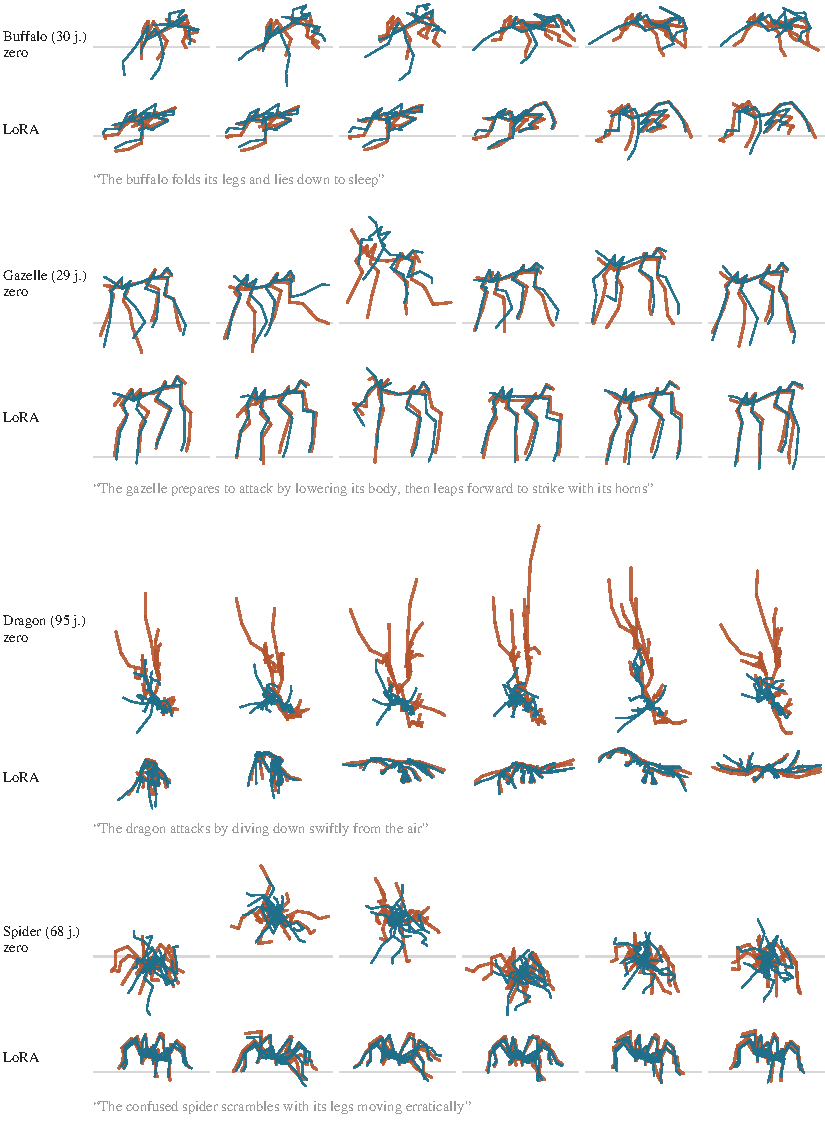
\includegraphics[width=\linewidth]{figures/tb_filmstrips.pdf}
\caption{Truebones arms of Table~\ref{tab:lora}: one held-out clip per rig, six frames spread evenly
over the clip, three-quarter view; the quoted sentence is the conditioning prompt. In every panel the
directly predicted joint positions (clay) are overlaid by the forward kinematics of the predicted
rotations (teal); a visible separation is the projected FK--pose discrepancy (a single view can hide
a disagreement in depth). Rows: the library model with the rig's statistics only (\emph{zero}, the
unadapted snapshot, whereas the zero column of Table~\ref{tab:lora} is read after at most 15
warm-up steps) and the per-rig adapter (\emph{LoRA}). Frames are anchored on the root horizontally
and keep their height above the floor; the grey line marks the floor height beneath the root. The
Dragon, a flying rig, is anchored on the root in all axes, which removes its dive trajectory. Both
rows of a rig are drawn at the same scale.}\label{fig:tb_filmstrips}
\end{figure}

\section{Validation split}\label{app:split}

The library is split per rig: for every rig, \num{5}\% of its clips are assigned to validation by
a hash of the clip identifier (seed 42) and the rest to training, so that every rig with enough
clips is represented in both parts. The split is fixed before any model is trained and is shared by
the evaluator and by every generator and adapter in this paper; checkpoints are selected on the
validation loss. Validation holds \num{3{,}899} clips over \num{311} rigs and training
\num{73{,}995} clips. Retrieval pools are formed by chunking the validation set in dataset order
(rigs sorted by name), so a pool of 64 holds clips of one rig or of neighbouring rigs; the last
59 clips do not fill a pool and are excluded from the R-precision but not from the FID or the
matching score.

\paragraph{Pool size.} Retrieval among more candidates is harder for the real clips and for the
generated ones alike, and the pool size is a free parameter of the protocol. Table~\ref{tab:pool}
re-scores the same generated samples at four pool sizes; the ranking of the two models and their
distance to the real clips do not depend on the choice, and the main text uses 64.

\begin{table}[h]
\centering\small
\caption{R@1 of the same samples (20 steps, $s{=}2$, one seed) re-scored in pools of 16, 32, 64 and
128 formed by chunking the dataset order; the incomplete last pool is dropped. The real clips are scored
by the same evaluator in the same pools.}\label{tab:pool}
\begin{tabular}{lcccc}
\toprule
Pool size & 16 & 32 & 64 & 128 \\
Pools & 243 & 121 & 60 & 30 \\
\midrule
Real clips (reference) & \num{0.985} & \num{0.975} & \num{0.964} & \num{0.962} \\
\method{} (pilot, \num{36}M) & \num{0.938} & \num{0.918} & \num{0.897} & \num{0.891} \\
\method{} (\num{303}M) & \num{0.956} & \num{0.937} & \num{0.922} & \num{0.915} \\
\bottomrule
\end{tabular}
\end{table}
